\documentclass[unknownkeysallowed]{beamer}
\usepackage[french,english]{babel}

\usepackage{pythontex}
\usepackage[english]{babel}
\usepackage{listings}
\usepackage{xcolor}
\usepackage{movie15}
\usepackage{amssymb}
\usepackage{amsthm}
\usepackage{amsfonts}
\usepackage[utf8]{inputenc}
\usepackage{pythontex}
\usepackage{fontawesome}
\usetheme{Madrid}
\DeclareMathOperator*{\argmin}{arg\,min}
\usecolortheme{beaver}
\usepackage{utopia}%font utopia imported
\usepackage{graphicx}
\newtheorem{exmp}{Exemple}[section]
\usetheme{Boadilla}
\usepackage{amsmath}
\usepackage{stmaryrd}
\usecolortheme{beaver}
\renewcommand{\contentsname}{Table des matières} 

\begin{document}


%%%%%%%%%%%%%%%%%%%%%%%%%%%%%%%%%%%%%%%%%%%%%%%%%%%%%%%%%%%%%%%%%%%%%%%%%%%%%%%
%%%%%%%%%%%%%%%%%%%%%%             Headers               %%%%%%%%%%%%%%%%%%%%%%
%%%%%%%%%%%%%%%%%%%%%%%%%%%%%%%%%%%%%%%%%%%%%%%%%%%%%%%%%%%%%%%%%%%%%%%%%%%%%%%



%%%%%%%%%%%%%%%%%%%%%%%%%%%%%%%%%%%%%%%%%%%%%%%%%%%%%%%%%%%%%%%%%%%%%%%%%%%%%%%
\begin{frame}
\bigskip
\bigskip
\begin{center}{
\LARGE\color{marron}
\textbf{HMMA 307 : Modèle linéaire avancés}
\textbf{ }\\
\vspace{0.5cm}
}

\color{marron}
\textbf{Utilisation de la médiane géométrique et de l’estimation robuste dans des espaces de Banach}
\end{center}

\vspace{0.25cm}

\begin{center}
\textbf{Hanna Bacave \\}
\faGithub\href{https://github.com/hannabacave/geometric_median_estimation}{Geometric median estimation}
\\
\vspace{0.5cm}
Université de Montpellier \\
\end{center}

\centering

\includegraphics[width=0.13\textwidth]{Logo_université_montpellier.png}

\end{frame}
%%%%%%%%%%%%%%%%%%%%%%%%%%%%%%%%%%%%%%%%%%%%%%%%%%%%%%%%%%%%%%%%%%%%%%%%%%%%%%%



%%%%%%%%%%%%%%%%%%%%%%%%%%%%%%%%%%%%%%%%%%%%%%%%%%%%%%%%%%%%%%%%%%%%%%%%%%%%%%%
%%%%%%%%%%%%%%%%%%%%%%%%       PLAN      %%%%%%%%%%%%%%%%%%%%%%%%%%%%%%%%%%%%%%
%%%%%%%%%%%%%%%%%%%%%%%%%%%%%%%%%%%%%%%%%%%%%%%%%%%%%%%%%%%%%%%%%%%%%%%%%%%%%%%



%%%%%%%%%%%%%%%%%%%%%%%%%%%%%%%%%%%%%%%%%%%%%%%%%%%%%%%%%%%%%%%%%%%%%%%%%%%%%%%
\begin{frame}{Table of Contents}
\tableofcontents[hideallsubsections]
\end{frame}
%%%%%%%%%%%%%%%%%%%%%%%%%%%%%%%%%%%%%%%%%%%%%%%%%%%%%%%%%%%%%%%%%%%%%%%%%%%%%%%



%%%%%%%%%%%%%%%%%%%%%%%%%%%%%%%%%%%%%%%%%%%%%%%%%%%%%%%%%%%%%%%%%%%%%%%%%%%%%%%
\AtBeginSection[]
{
\begin{frame}<beamer>{Table of Contents}
\tableofcontents[currentsubsection,
    hideothersubsections,
    sectionstyle=show/shaded,
]
\end{frame}
}
%%%%%%%%%%%%%%%%%%%%%%%%%%%%%%%%%%%%%%%%%%%%%%%%%%%%%%%%%%%%%%%%%%%%%%%%%%%%%%%




%%%%%%%%%%%%%%%%%%%%%%%%%%%%%%%%%%%%%%%%%%%%%%%%%%%%%%%%%%%%%%%%%%%%%%%%%%%%%%%
%%%%%%%%%%%%%%%%%%%%%%%%%%%%%%%%%%%%%%%%%%%%%%%%%%%%%%%%%%%%%%%%%%%%%%%%%%%%%%%
\section{Régression quantile}
\label{sec:Régression quantile}
%%%%%%%%%%%%%%%%%%%%%%%%%%%%%%%%%%%%%%%%%%%%%%%%%%%%%%%%%%%%%%%%%%%%%%%%%%%%%%
%%%%%%%%%%%%%%%%%%%%%%%%%%%%%%%%%%%%%%%%%%%%%%%%%%%%%%%%%%%%%%%%%%%%%%%%%%%%%%%

%%%%%%%%%%%%%%%%%%%%%%%%%%%%%%%%%%%%%%%%%%%%%%%%%%%%%%%%%%%%%%%%%%%%%%%%%%%%%%%

%%%%%%%%%%%%%%%%%%%%%%%%%%%%%%%%%%%%%%%%%%%%%%%%%%%%%%%%%%%%%%%%%%%%%%%%%%%%%%%

%%%%%%%%%%%%%%%%%%%%%%%%%%%%%%%%%%%%%%%%%%%%%%%%%%%%%%%%%%%%%%%%%%%%%%%%%%%%%%%
\begin{frame}
\frametitle{Définitions}
\begin{block}{Médiane}
Soit $y_1, ..., y_n \in \mathbb{R}$, on définit la \textit{médiane} [1] par :
$$Med_{n}(y_1, ..., y_n) \in \argmin_{\mu \in \mathbb{R}} \frac{1}{n} \sum\limits_{i=1}^{n} | y_i - \mu |.$$
\end{block}
\vspace{0.5cm}
\textbf{Rq.} En pratique, on utilise des façons plus simples pour calculer la médiane, mais celles-ci ne sont pas adaptées aux dimensions supérieures à 1.
\end{frame}

%%%%%%%%%%%%%%%%%%%%%%%%%%%%%%%%%%%%%%%%%%%%%%%%%%%%%%%%%%%%%%%%%%%%%%%%%%%%%%

\begin{frame}
\frametitle{Definitions}
\begin{itemize}
    \item $y_1, ..., y_n \in \mathbb{R}$ observations,
    \item $x_1, ..., x_n \in \mathbb{R}^p$ variables explicatives.
\end{itemize}
\vspace{0.1cm}
\begin{block}{Régression quantile}
Soit $\alpha \in ]0,1[$, on appelle \textit{régression quantile} [1] les coefficients :
$$\beta^{\alpha} \in \argmin\limits_{\beta \in \mathbb{R}^p} \frac{1}{n} \sum\limits_{i=1}^{n} l_{\alpha}(y_i - x_i^T\beta),$$
où 
$$X = \begin{pmatrix}
x_1^T \\
x_2^T \\
\vdots\\
x_n^T
\end{pmatrix} 
\in \mathbb{R}^{nxp}.$$
\end{block}
\end{frame}

%%%%%%%%%%%%%%%%%%%%%%%%%%%%%%%%%%%%%%%%%%%%%%%%%%%%%%%%%%%%%%%%%%%%%%%%%%%%%%%%%%%%%%%%%%%%%%%%%%%%%%%%%%%%%%%%%%%%%%
\begin{frame}
\frametitle{Première comparaison - Régression quantile et régression linéaire}
\begin{figure}[!h]
    \begin{center}
   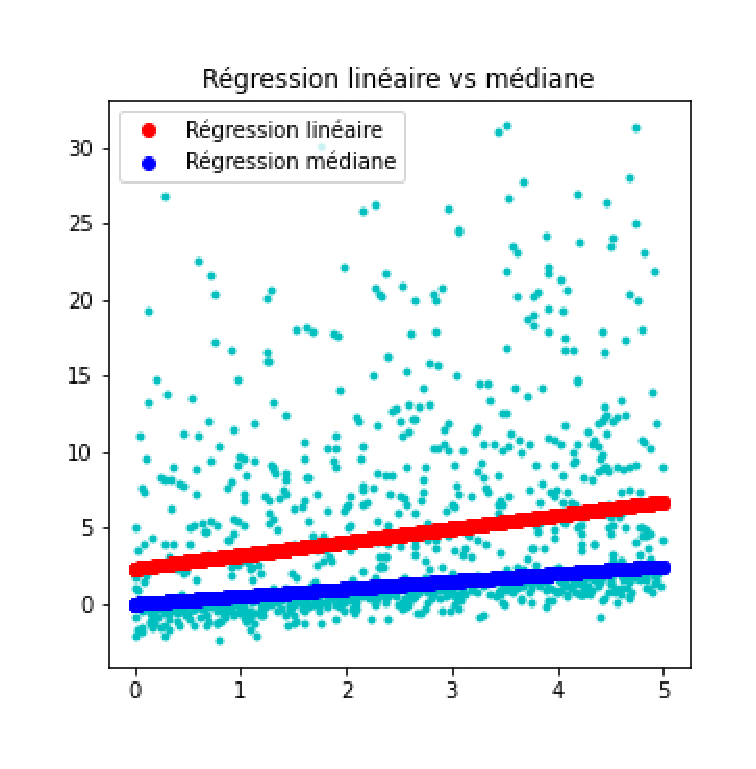
\includegraphics[width=7cm]{reg1.pdf}
   \end{center}
    \end{figure}
\end{frame}


%%%%%%%%%%%%%%%%%%%%%%%%%%%%%%%%%%%%%%%%%%%%%%%%%%%%%%%%%%%%%%%%%%%%%%%%%%%%%%%%%%%%%%%%%%%%%%%%

\section{Régression quantile en grande dimension avec des données sparses}

%%%%%%%%%%%%%%%%%%%%%%%%%%%%%%%%%%%%%%%%%%%%%%%%%%%%%%%%%%%%%%%%%%%%%%%%%%%%%%%
%%%%%%%%%%%%%%%%%%%%%%%%%%%%%%%%%%%%%%%%%%%%%%%%%%%%%%%%%%%%%%%%%%%%%%%%%%%%%%%
\begin{frame}
\frametitle{Présentation de la procédure - 1}
\begin{block}{Présentation du problème}
On voudrait résoudre le problème d'optimisation [2] suivant :
$$Y_j = \lambda_0^T x_j + \epsilon_j$$
où 
\begin{itemize}
    \item $\epsilon_j$ est un vecteur iid de moyenne $0$, mais n'est pas gaussien ;
    \item $\lambda_0$ est un vecteur sparse, c'est-à-dire que la dimension s du support de $\lambda_0$ est très nettement inférieure à D ;
    \item $D >> n$
\end{itemize}
\end{block}

\end{frame}

%%%%%%%%%%%%%%%%%%%%%%%%%%%%%%%%%%%%%%%%%%%%%%%%%%%%%%%%%%%%%%%%%%%%%%%%%%%%%%%
\begin{frame}
\frametitle{Présentation de la procédure - 2}
\begin{enumerate}
    \item On commence par définir : 
    \begin{itemize}
        \item $t > 0$ fixé, 
        \item $k = \floor{3.5t} + 1$
        \item $m = \floor{\frac{n}{k}}$
    \end{itemize}
    Pour $1 \leq l \leq k$, on définit $G_l = \{(l-1)m + 1, ..., lm \}$ et 
\begin{center}
    $\mathbb{X}_l = (x_{j_1} | ... | x_{j_m}),$ où,  $j_i = (l - 1)m + i \in G_l$.
\end{center}
    \item On calcule :
    $$\hat{\lambda}_\epsilon^l = \argmin\limits_{\lambda \in \mathbb{R}^D} \left[ \frac{1}{|G_l|} \sum\limits_{j \in G_l} (Y_j - \lambda^T x_j)^2 + \epsilon \|\lambda\|_1 \right]$$.
    \item Enfin, on prend :
    $$\hat{\lambda}_\epsilon^* = med(\hat{\lambda}_\epsilon^1, ..., \hat{\lambda}_\epsilon^k),$$
\end{enumerate}
\end{frame}

%%%%%%%%%%%%%%%%%%%%%%%%%%%%%%%%%%%%%%%%%%%%%%%%%%%%%%%%%%%%%%%%%%%%%%%%%%%%%%%
\begin{frame}
\frametitle{Comparaisons des estimateurs}
\begin{block}{Méthode utilisée}
On utilise le critère du $R^2$ pour comparer les estimateurs.
\end{block}
\begin{figure}[!h]
    \begin{center}
     \caption{\label{étiquette}Comparaisons entre l'estimateur "Lasso médian" et d'autres estimateurs.}
   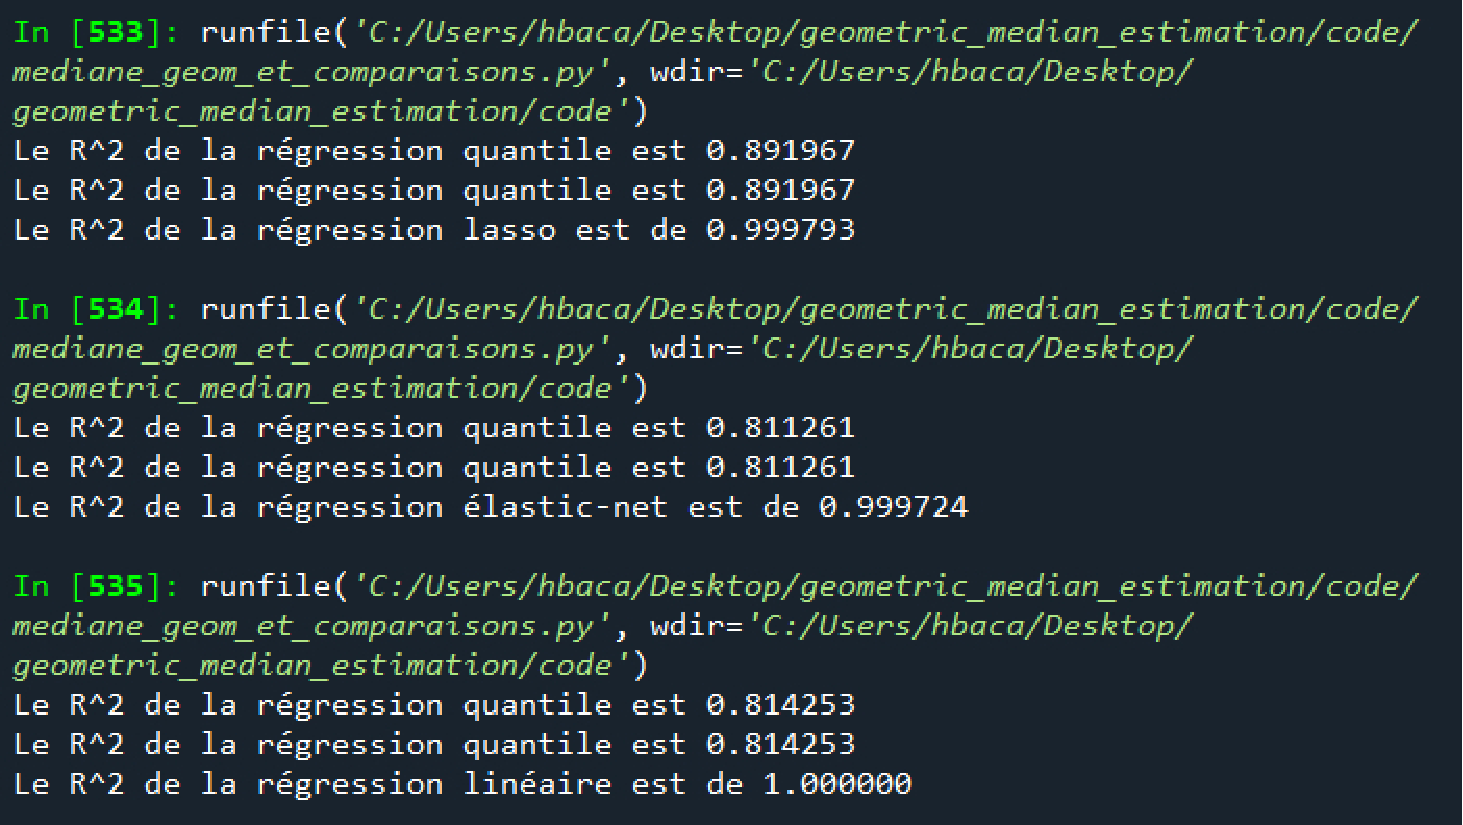
\includegraphics[width=8cm]{comparaisons.pdf}
   \end{center}
    \end{figure}

\end{frame}

%%%%%%%%%%%%%%%%%%%%%%%%%%%%%%%%%%%%%%%%%%%%%%%%%%%%%%%%%%%%%%%%%%%%%%%%%%%%%%%

\begin{frame}{Conclusion}
\begin{block}{Les principales difficultés rencontrées}
\begin{itemize}
    \item Compréhension du modèle ;
    \item Simulation des variables ;
    \item Utilisation de la médiane géométrique par le biais de la régression quantile.
\end{itemize}
\end{block}
\vspace{0.5cm}
\begin{block}{Pour aller plus loin}
\begin{itemize}
    \item Comparaisons des erreurs sur des histogrammes par le biais de la validation croisée ;
    \item Optimisation du code.
\end{itemize}
\end{block}
\end{frame}

 %%%%%%%%%%%%%%%%%%%%%%%%%%%%%%%%%%%%%%%%%%%%%%%%%%%%%%%%%%%%%%%%%%%%%%%%%%%%%
  %%%%%%%%%%%%%%%%%%%%%%%%%%%%%%%%%%%%%%%%%%%%%%%%%%%
\begin{frame}{Bibliographie}
[1] Joseph Salmon, \textit{Modéle linéaire avancé : Régression Quantile}, 2019, \url{http://josephsalmon.eu/enseignement/Montpellier/HMMA307/RegressionQuantile.pdf} ; 

[2] Stanislav Minsker, \textit{Geometric median and robust estimation in Banach spaces}, 2015, \url{https://arxiv.org/pdf/1308.1334.pdf}. 

\printbibliography
\end{frame}
 %%%%%%%%%%%%%%%%%%%%%%%%%%%%%%%%%%%%%%%%%%%%%%%%%%%%%%%%%%%%%%%%%%%%%%%%%%%%%



\end{document}